%%%%%%%%%%%%%%%%%%%%%%%%%%%%%%%%%%%%%%%%%%%%%%%%%%%%%%%%%%%%%%%%%%%%%%%%%%%%%%%%
%2345678901234567890123456789012345678901234567890123456789012345678901234567890
%        1         2         3         4         5         6         7         8

\documentclass[letterpaper, 10 pt,noend]{article}  % Comment this line out if you need a4paper

%\documentclass[a4paper, 10pt, conference]{ieeeconf}      % Use this line for a4 paper

%\IEEEoverridecommandlockouts                              % This command is only needed if 
                                                          % you want to use the \thanks command

%\overrideIEEEmargins                                      % Needed to meet printer requirements.

% See the \addtolength command later in the file to balance the column lengths
% on the last page of the document

% numbers option provides compact numerical references in the text. 

\usepackage[hidelinks, bookmarks=true]{hyperref}
\usepackage[font=small,labelfont=bf]{caption}

% The following packages can be found on http:\\www.ctan.org
\usepackage{graphics} % for pdf, bitmapped graphics files
\usepackage{epsfig} % for postscript graphics files
\usepackage{amsmath} % assumes amsmath package installed
\usepackage{amssymb}  % assumes amsmath package installed
\usepackage{listings}
\usepackage{graphicx,float,wrapfig}
\usepackage{subfig}
\usepackage{algpseudocode}
\usepackage{algorithm}
\usepackage{mathtools}
\usepackage{cite}
\usepackage{color}
\usepackage[usenames,dvipsnames,svgnames,table]{xcolor}
\usepackage[inline,shortlabels]{enumitem}

%% Define symbols and special formats for texts
\DeclareMathOperator{\F}{\rotatebox[origin=c]{45}{$\Box$}}
\DeclareMathOperator{\G}{\Box}
\DeclareMathOperator{\X}{\bigcirc}
\DeclareMathOperator{\Cox}{\scalebox{0.8}{$\F$}\hspace{-9.3pt}\bigcirc}
\newcommand{\NN}{\mathbb{N}}
\newcommand{\FALSE}{\mathbf{false}}
\newcommand{\TRUE}{\mathbf{true}}
\newcommand{\TODO}[1]{{\color{red}#1}}

\title{\LARGE \bf CS 6751 Intro to Mobile Robot Manipulation Project Proposal}


\author{Scott Hamill, Gangyuan Jing, Kai Weng Wong% <-this % stops a space
}


\begin{document}


\maketitle
\thispagestyle{empty}
\pagestyle{empty}

% add our sections here
\section{Introduction and Background}


Creating robot controllers by combining high-level task planning with low level motion planning has been a topic of recent interest \cite{HKG2009,Belta2008,Bhatia2011,Dornhege2009,Erdem2011,Tom2014,Srivastava2014}.
The integration of discrete task reasoning and motion planning allows users to specify complex robot behaviors and tasks from a high-level perspective while satisfying low level motion constraints.

Past research has shown promising results on controller synthesis with formal methods \cite{HKG2009,Belta2008,Bhatia2011,Wongpiromsarn,Maly,Vasile}.
Recent research has addressed controller synthesis using formal methods, specifying tasks and behaviors in a formal language such as Linear Temporal Logic (LTL) \cite{HKG2009,Belta2008,Bhatia2011,Dornhege2009,Erdem2011,Tom2014,Srivastava2014}.
Controllers synthesized in this manner are correct-by-construction, thereby providing guarantees on the behavior of the robot.
These algorithms typically abstract the robot system and environment by discretizing the workspace.
This technique works well for mobile robot systems, but discretizations for manipulation systems are typically intractable due to combinatorial blow-up of the state space.

Formal methods have previously been applied to controller synthesis for manipulation \cite{Dornhege2009,Erdem2011,Tom2014,Srivastava2014,CambonAG09,KaelblingL11,PlakuH10,HeLKV15}.
Most of these works utilize AI based planners for high-level task planning and low-level motion planners for finding feasible robot trajectories \cite{Nau,Hoffmann01}.
While these frameworks allow users to specify high-level behaviors and task specifications, the resulting behaviors are non-reactive in that the robot behavior does not depend on the state of the environment.

This work addresses synthesizing correct-by-construction controllers for a manipulation task from a high-level behavioral specification.
This framework provides three main contributions: a high-level {\it task planner} for determining sequences of high-level actions, a {\it trajectory planner} for finding and executing feasible manipulator motions, and an {\it action planner} for performing precise manipulator motion and actuation.
This framework is is demonstrated on a Baxter robot (Rethink Robotics) assembling a series of modular robot components into a pre-defined configuration. 


\begin{comment}
With the development of hardware and software of robots,
There is an increasing interest in combining high-level task planning
with low-level motion planning when creating robot controllers \cite{HKG2009,Belta2008,Bhatia2011,Dornhege2009,Erdem2011,Tom2014,Srivastava2014}.
While integrating tasking and motion planning enables users to specify complex robot tasks from a high-level perspective,
combining discrete task reasoning with continuous motion planning brings challenges to designing robot controllers.

Past research has shown promising results on controller synthesis with formal methods \cite{HKG2009,Belta2008,Bhatia2011,Wongpiromsarn,Maly,Vasile}.
In these papers, robot tasks are expressed in formal language such as Linear Temporal Logic (LTL).
Controllers can be automatically synthesized from the task specification,
while providing guarantees on the correctness of robot behaviours.
These controller synthesis algorithms typically abstract robot systems and environment by discretizing the robot workspace,
in order to avoid the combinatorial blow up of the state space.
While the abstraction reduces the complexity of mobile systems,
the discretization is usually intractable for manipulation systems,
due to high degrees of freedom of manipulation tasks.

Many frameworks were developed on controller synthesis with formal methods for manipulation \cite{Dornhege2009,Erdem2011,Tom2014,Srivastava2014,CambonAG09,KaelblingL11,PlakuH10,HeLKV15}.
Most of these works utilize AI based planners for high-level task planning and low-level motion planners for finding feasible robot trajectories \cite{Nau,Hoffmann01}.
These frameworks allows user to control manipulation systems with high-level task specifications.
However, high-level planners used in these frameworks limit possible tasks to non-reactive,
i.e. the behavior of the robot does not depend on the state of the environment.

Moreover, formal methods are also used in robotics to generate controllers for coordination of a team of robots \cite{ChenDSB12,KaramanF08,GuoTD14,VasileB14}.
In these work, tasks are specified in Temporal Logic and controllers are automatically synthesized and distributed to each robot agent. 
However, little work has been done on task and motion planning for multi-agent manipulation system with formal method.

In this work, we are interested in developing a framework for automatically synthesizing correct-by-construction controllers
for multi-agent manipulation tasks expressed in Linear Temporal Logic. The framework consists of three main components:
a high-level \textit{task planner} for generating and distributing controllers to each agent,
a \textit{trajectory planner} for finding feasible path and moving each manipulator while avoiding collisions,
and and \textit{action planner} for creating precise motion and actuation for each manipulator.
The framework will be demonstrated with an experiment of two physical Baxter robots assembling a set of modular robots. 
\end{comment}

\section{Task Planning}
The task planner in this work is based on the framework introduced in (\TODO{hadas paper}).
\begin{itemize}
\item Change specification language for multirobot
\item How to distribute tasks from a single automaton
\item How to deal with the situation when the trajectory planner returns not path?
\end{itemize}
\section{Trajectory Planning (Catherine)}

This component is divided into two subsections:
\begin{enumerate}%[label=\thesection.\arabic*]
\item Trajectory Planner for robot arm trajectory planning, and
\item Trajectory Executor for robot arm trajectory execution.
\end{enumerate}

\subsection{Trajectory Planner}

During execution, the task planner requests the path planner to create trajectory plans for one or more robot arms. The planner aims to find a plan that (i) each arm starts at its initial configuration, and (ii) each arm ends with each robot end effector within a certain radius from the final desired workspace position. If the planner finds a plan, it returns the joint-space trajectory for each arm. If the planning exceeds the time limit, then the planner aborts and returns no trajectories. 

There are a variety of path planning algorithms developed in the community~\cite{DBLP:books/daglib/0016830} and some algorithms are adapted for finding robot arm trajectories. 
Researchers have proposed sampling-based approaches with probabilistic completeness such as the Rapidly-Exploring Random Tree (RRT) algorithm ~\cite{VahrenkampBAKD09} to find trajectories for robot arms. Others have used Probabilistic RoadMaps (PRM) that work with high-dimensional spaces~\cite{KavrakiSLO96} but the algorithm requires pre-computation of the roadmap and no dynamic obstacles in the environment. In this project, we will not conduct pre-processing and the other arms can become obstacles so we are using RRT to find trajectories for the robot arms.

First, we plan to try two different RRT approaches and compare their performance. With RRT, there are still multiple ways to generate a trajectory plan.
One of them is to generate trajectory plan synchronously.
For example, if there are four arms available for a task, or two Baxters, then the planning could be synchronous, i.e, we plan all the arms at the same time and each node in RRT stores the joint information of the four arms. With each arm having 7 degrees of freedom (DoF), a synchronous planning has up to 28 degrees of freedom.
With this approach, assuming the workspace has no other obstacles, collision avoidance with the other arms is taken care of during the planning phase so it is unnecessary during trajectory execution.  
The trade off of synchronous planning is that one arm may wait for the others even though its trajectory is found.

Alternatively, another way would be to first create a plan each arm separately and assign priorities to each arm. An arm then replans only when its trajectory intersects with the plan of another arm with a higher priority. Compared with the synchronous approach, each planning contains 7 degrees of freedom but re-plannings of trajectory can go up to (n-1) times, with n being the number of arms. 

Second, we plan to create our own version of RRT planner and also utilize off-the-shelf library with RRT such as the Open Motion Planning library (OMPL)~\cite{sucan2012the-open-motion-planning-library} to find out the one with better performance.
Compared with creating our own RRT planner, OMPL has lots of planning algorithms available, but most examples of OMPL work with single robot or arm and planning for multiple arms simultaneously with OMPL may be unfeasible. We plan to learn more about OMPL and then decide if we are creating our own RRT planner or we are using OMPL to build our planner.

Finally, RRT is only a template for planning and we need to complete the template with ways to propagate a trajectory and smoothen the resulting trajectory. 
During the planning phrase, we plan to optimize the final trajectory by reducing the difference in joint angles between two nodes in the RRT tree. We use inverse kinematics find robot joint angles given a desired location of the end effector.


%To conduct a path planning of the robot arms, the planner takes in:

%\begin{itemize}
%\item the number of arms we are planning, 
%\item the starting joint configurations of each arm, and
%\item the final workspace positions of robot end effectors.
%\end{itemize}

two-step planning


\subsection{Trajectory Executor}

Besides a trajectory planner, the person in charge of this component also creates a trajectory executor that executes any given trajectory.
Once the task planner receives a plan, it can invoke the trajectory executor to execute the path. The executor takes in a joint-space trajectory and notifies the task planner when it finishes the execution. The task planner then invokes planning by the action planner in the next section to conduct fine and accurate objects manipulation.

\section{Experiment}

We conducted an experiment of our system with a Rethink Baxter robot and six wooden modules with AprilTags on them. For sensing and localization of the modules, we used the camera on Baxter's left hand and an external Kinect. In this experiment, we started from some random location of the six modules (Fig.~\ref{fig:initConfig}) and tried to form a snake configuration with the six modules (Fig.~\ref{fig:finalConfig}).
The link to a video of the experiment is \url{https://youtu.be/OXdHslVxjws}. 

\begin{figure}[ht!]%[H]
\centering
\subfloat[Inital position of the modules]{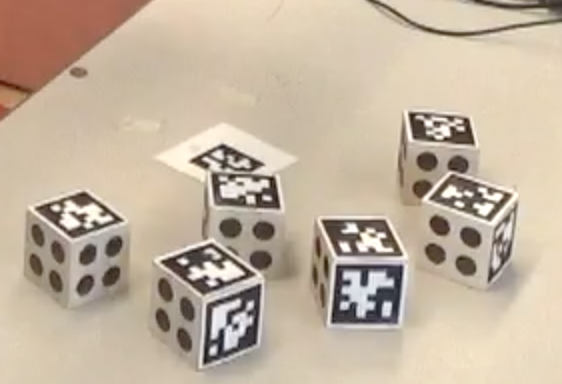
\includegraphics[width=0.45\columnwidth]{pics/init_module_location.png}\label{fig:initConfig}}
\quad
\subfloat[Final module configuration]{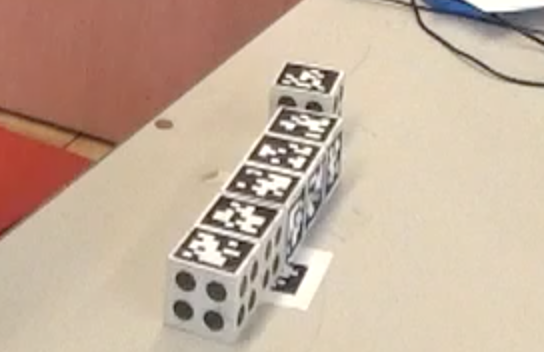
\includegraphics[width=0.45\columnwidth]{pics/snake_modules.png}\label{fig:finalConfig}}\\
\caption{Final Module Configuration}
\end{figure}

In this experiment, our system was able to recover from grasping failure and our system continued to finish the assembly with the instructions from the high-level planner. As shown in Table~\ref{table:result}, out of the five connections between the modules, our system successfully performed 3 connections: connected the third, the fourth and fifth module to the assembly. Our system failed to connect the second module to the first one due to misalignment and it also failed to connect the last module to the assembly due to too small of a motion. 


%\begin{center}
\begin{table}[h]
\caption{Connection Result of Modules} %F for Failed and S for Succeeded}
\begin{tabular}{|c |c |c |c |c |c|}
\hline
 Connection &  1-2 & 2-3 & 3-4 & 4-5 & 5-6 \\\hline 
  Result  & failed & succeeded & succeeded & succeeded & failed \\\hline  
\end{tabular}\label{table:result}
\end{table}
%\end{center}

In the future, we will improve the fine adjustment to connect the modules. We also want to conduct synthesis of the trajectory planner. We will use the right arm to localize and manipulate the modules. We plan to attempt more complex configuration to showcase the capabilities of our system.




\bibliographystyle{plain}
\bibliography{ref}

\end{document}
